%% Supplementary Information for the AVB-Engage manuscript (JAIHC). Compile with pdfLaTeX alongside sn-jnl.cls.
%% Holds the material moved out of the main text on 2026-11-03: the decoding rules and training objective
%% (main-text Section 3.1) the evaluation metrics (main-text Section 4.4), and, on 2026-11-09, the threshold search, the pre-training stages, the training-variable sweep, the training configuration, the per-level results and the behavior-branch table.
\documentclass[pdflatex,sn-basic]{sn-jnl}

\usepackage{amsmath,amssymb,amsfonts}
\usepackage{graphicx}
\usepackage{xcolor}
\usepackage{booktabs}
\usepackage{algorithm}
\usepackage{algorithmicx}
\usepackage{algpseudocode}
\usepackage{tikz}
\usepackage{pgfplots}
\pgfplotsset{compat=1.17}
% Shared figure colours (validated for colour-vision deficiency; see dataviz palette).
\definecolor{ours}{HTML}{2A78D6}      % our single models
\definecolor{fused}{HTML}{EB6834}     % our late fusion
\definecolor{published}{HTML}{8F8E88} % published EngageNet baselines
\definecolor{inkmuted}{HTML}{52514E}
\definecolor{boxfill}{HTML}{F3F2EF}
\definecolor{seqlo}{HTML}{FFFFFF}
\definecolor{seqhi}{HTML}{104281}


\newcommand{\ournet}{AVB-Engage}
\renewcommand{\thesection}{S\arabic{section}}
\renewcommand{\theequation}{S\arabic{equation}}
\renewcommand{\thetable}{S\arabic{table}}
\renewcommand{\thefigure}{S\arabic{figure}}
\renewcommand{\thealgorithm}{S\arabic{algorithm}}

\raggedbottom

\begin{document}

\title[Supplementary Information]{Supplementary Information for ``\ournet: Audio-Visual and Facial-Behavior Fusion for Ordinal Student Engagement Recognition''}

\author*[1]{\fnm{First} \sur{Author}}\email{first.author@example.edu}
\author[1]{\fnm{Second} \sur{Author}}
\author[1]{\fnm{Third} \sur{Author}}
\affil*[1]{\orgdiv{Department}, \orgname{Organization}, \orgaddress{\city{City}, \state{State}, \country{Country}}}

\abstract{Online Resource 1 for the article ``\ournet: Audio-Visual and Facial-Behavior Fusion for Ordinal Student Engagement Recognition'', submitted to the \emph{Journal of Ambient Intelligence and Humanized Computing}. This document supplements the main article. Section~S1 gives the decoding rules and the training objective summarized in Section~3.1 of the main text; Section~S2 defines the four evaluation metrics named in Section~4.4; Section~S3 gives the layer-by-layer configuration of the cross-attention fusion of Section~3.2.4; Section~S4 lists the training and inference procedure; and Sections~S5 to S7 hold the full tables of the segment-count and training-variable ablations, the fusion-weight sweep, the computational cost, and the label-granularity analysis referred to in Section~5.}

\maketitle

\section{Decoding rules and training objective}\label{sec:s_formulation}

Each sample is a clip of a student's webcam recording with face frames, an audio track and a per-frame facial-behavior descriptor. The label set is $\mathcal{Y} = \{0, 1, \ldots, K-1\}$ with $K = 4$, where larger values mean higher engagement. For a clip with label $y$, a model produces logits $z \in \mathbb{R}^{K}$ and class probabilities $p_k = \exp(z_k) / \sum_{j} \exp(z_j)$. The usual decision rule takes the largest probability,
\begin{equation}
\hat{y} = \arg\max_{k} \; p_k \label{eq:s_argmax}
\end{equation}
Here, $\hat{y}$ is the predicted level. This rule uses the value of each probability but not the position of each class on the scale. In order to use the position of each class, the ordered alternative used in the main text first reduces the probability vector to the expected level,
\begin{equation}
\mu = \sum_{k=0}^{K-1} k \, p_k \label{eq:s_mu}
\end{equation}
Here, $\mu$ is a continuous value in $[0, K-1]$. The expected level is then cut with increasing thresholds $\tau_1 < \tau_2 < \tau_3$, and the predicted level is
\begin{equation}
\hat{y} = \sum_{m=1}^{K-1} \mathbf{1}\!\left[\mu \geq \tau_m\right] \label{eq:s_thresh}
\end{equation}
Here, $\mathbf{1}[\cdot]$ is the indicator function, so $\hat{y}$ is the number of thresholds that $\mu$ reaches. The thresholds are fitted on the validation split and are not learned during training. The fit is a coordinate search: starting from $(0.5, 1.5, 2.5)$, each threshold in turn is moved over a window of $\pm 1.0$ in steps of 0.01 while the other two are held fixed and the order of the thresholds is kept, for three rounds, and the setting with the highest validation top-1 accuracy is retained, with ties broken by adjacent accuracy and then by mean absolute error.

During training, the order of the levels is used by adding to the cross-entropy loss $\mathcal{L}_{\mathrm{CE}}$ a penalty that grows with the distance between the predicted and the true level,
\begin{equation}
\mathcal{L} = \mathcal{L}_{\mathrm{CE}} + \lambda \sum_{k} p_k \left| c_k - c_y \right|, \qquad c_k = \frac{k}{K-1} \label{eq:s_loss}
\end{equation}
Here, $c_y$ is the position of the true level $y$, the class positions $c_k$ are normalized to $[0,1]$, and $\lambda$ sets the weight of the distance term; both terms are averaged over the mini-batch. The audio-visual network ($\lambda = 0.15$) and the segment-Transformer model are trained with (\ref{eq:s_loss}), and the fused class probabilities are decoded with (\ref{eq:s_mu}) and (\ref{eq:s_thresh}) instead of (\ref{eq:s_argmax}).

\emph{Threshold search.} The thresholds of the fused vector are fitted on the validation split by a coordinate search: starting from $(0.5, 1.5, 2.5)$, each threshold in turn is moved over a window of $\pm 1.0$ in steps of 0.01 while the other two are held fixed and the order of the thresholds is kept, for three rounds, and the setting with the highest validation top-1 accuracy is retained, with ties broken by adjacent accuracy and then by mean absolute error. For the network alone, four decoders are compared in Section~5.3 of the main text: argmax; argmax after a per-class logit bias fitted on validation (a grid from $-2$ to $2$ in steps of 0.1 for levels 1--3, with level 0 fixed at 0); expected-level thresholds fitted on a grid with step 0.05; and refined expected-level thresholds obtained by a local search with radius 0.15 and step 0.005.

\section{Evaluation metrics}\label{sec:s_metrics}

Let $N$ be the number of test clips, with true levels $y_i$ and predictions $\hat{y}_i$, and let $\mathbf{1}[\cdot]$ denote the indicator function. Top-1 accuracy is the fraction of test clips whose predicted level matches the annotated level,
\begin{equation}
\mathrm{Top\text{-}1} = \frac{1}{N} \sum_{i=1}^{N} \mathbf{1}[\hat{y}_i = y_i].
\label{eq:s_top1}
\end{equation}
It scores a prediction one level from the truth in the same way as a prediction three levels from the truth. Adjacent accuracy is the fraction of clips predicted within one level of the truth,
\begin{equation}
\mathrm{Adj} = \frac{1}{N} \sum_{i=1}^{N} \mathbf{1}[|\hat{y}_i - y_i| \leq 1].
\label{eq:s_adj}
\end{equation}
The mean absolute error is the average distance in levels between the prediction and the truth,
\begin{equation}
\mathrm{MAE} = \frac{1}{N} \sum_{i=1}^{N} |\hat{y}_i - y_i|,
\label{eq:s_mae}
\end{equation}
so a value of 0.40 means that a prediction is on average 0.40 levels from the truth. Macro-F1 is the unweighted mean of the per-level F1 scores,
\begin{equation}
\mathrm{F1}_k = \frac{2\,P_k R_k}{P_k + R_k}, \qquad \mathrm{Macro\text{-}F1} = \frac{1}{K} \sum_{k=0}^{K-1} \mathrm{F1}_k,
\label{eq:s_f1}
\end{equation}
where $P_k$ and $R_k$ are the precision and recall of level $k$ and $K = 4$ is the number of levels. Because it weights the four levels equally, it cannot be raised by predicting the majority level. High values are preferred for top-1, adjacent accuracy and macro-F1, and a low value for MAE.

\section{Temporal alignment and cross-attention blocks}\label{sec:s_xattn}

\emph{Per-sample temporal alignment} (Section~3.1.3 of the main text). The valid audio steps of every sample are pooled onto the valid visual length of the same sample,
\begin{equation}
\begin{split}
\tilde{\mathbf{A}}_1[:, j] &= \frac{1}{|S_j|}\sum_{t \in S_j} \mathbf{A}_1[:, t],\\
S_j &= \left\{ t : \left\lfloor \tfrac{(j-1)L_a}{T_v} \right\rfloor \le t < \left\lceil \tfrac{j L_a}{T_v} \right\rceil \right\}
\end{split}
\end{equation}
Here, $\tilde{\mathbf{A}}_1[:, j]$ is the $j$-th aligned audio token for $j = 1, \dots, T_v$, $L_a$ and $T_v$ are the numbers of valid audio steps and valid visual tokens of the sample, the valid audio steps are indexed $t = 0, \dots, L_a - 1$, and $S_j$ is the $j$-th window under the rule of adaptive average pooling: the windows are of nearly equal width, and adjacent windows may share one step. Padding steps are excluded before pooling and masked afterwards, and $\tilde{\mathbf{A}}_1 \in \mathbb{R}^{128 \times 50}$ for a full clip.

\emph{Cross-attention blocks.} This section gives the configuration of the three cross-attention exchanges of the audio-visual network summarized in Section~3.1.4 of the main text. In the first and third exchanges, the attention is wrapped in a cross-attention block: layer normalization is applied to the query stream and to the key--value stream before the attention, the query, key and value projections have no bias, and the attended output is layer-normalized, passed through a two-layer feed-forward network (hidden width $2d_o$, GELU activation) and added back to itself. Each block projects to the width of its query stream, so $d_o = 128$ when the audio tokens are the queries and $d_o = 64$ when the first-stage visual tokens are the queries, and no dropout is used inside the blocks. The three exchanges are as follows.

\emph{First exchange.} The aligned audio tokens query the visual tokens and the visual tokens query the audio tokens, with $X_a = \tilde{\mathbf{A}}_1$ and $X_v = \mathbf{V}_1$ in the two cross-attention equations of the main text; the block outputs are added to the streams as the two cross-attention equations in Section~3.1.4 of the main text state.

\emph{Second stage and second exchange.} Each stream then passes through a second convolutional stage. Two one-dimensional convolution blocks (128$\to$256$\to$128, each with batch normalization, ReLU and max pooling with window 2) bring the audio tokens to $\mathbf{A}_2 \in \mathbb{R}^{128 \times 12}$, and two convolution blocks without pooling (64$\to$128$\to$128) bring the visual tokens to $\mathbf{V}_2 \in \mathbb{R}^{128 \times 50}$. In the second exchange, a standard multi-head attention layer in each direction, with biased projections and without the normalization and feed-forward sub-layers of the blocks above, lets the 12 audio tokens attend to the 50 visual tokens and the reverse; the attended output passes through dropout of 0.1 and is added to the stream.

\emph{Third exchange and pooling.} A final pair of cross-attention blocks forms the third exchange, this time without a residual connection: the audio stream is replaced by the output of the block in which the audio tokens are the queries and the visual tokens supply the keys and values, and the visual stream is replaced by the output of the reverse block. Each stream therefore ends as a summary of the other stream, weighted by the attention of its own tokens. Each stream is reduced over time to a 128-dimensional vector by masked attention pooling, in which a linear layer scores each valid time step and the tokens are averaged under the softmax of these scores. The two vectors are concatenated into the audio-visual summary $\mathbf{z} \in \mathbb{R}^{256}$, and a linear layer maps $\mathbf{z}$ to the four class probabilities $p_{\mathrm{AV}}$.

\section{Training and inference procedure}\label{sec:s_alg}

Algorithm~\ref{alg:s_ournet} lists the training and inference steps of \ournet{} in order. Before the fine-tuning reported in the main text, the audio-visual network was trained on EngageNet in three stages starting from the AffectNet initialization of the visual backbone, with the audio and fusion modules initialized randomly: 30 epochs with the cross-entropy loss at a learning rate of $10^{-2}$ and batch size 2, then 25 epochs with the ordinal objective at $10^{-4}$ and batch size 2, and then 8 epochs with the ordinal objective at $5 \times 10^{-5}$ and batch size 8, each stage starting from the weights of the previous one. These stages read every face frame of a clip; the class-balanced sampler was used in the reported fine-tuning only. All reported networks are fine-tuned from the resulting checkpoint with three random seeds, about 32 minutes per run on one NVIDIA RTX 3090 GPU with 24\,GB of memory; the segment Transformer was trained on the same GPU and the gradient-boosting model on the CPU, both on the training split only.

\begin{algorithm}[t]
\caption{\ournet{} training and inference}\label{alg:s_ournet}
\begin{algorithmic}[1]
\Require face frames $\mathbf{I}$, log-mel spectrogram $\mathbf{X}_a$, OpenFace series $\mathbf{B}$, level $y$
\Ensure engagement level $\hat{y} \in \{0,1,2,3\}$
\For{each training iteration}
\State $\mathbf{V}_1 \gets \mathrm{Conv1D}(\mathrm{EfficientFace}(\mathbf{I}))$
\State $\tilde{\mathbf{A}}_1 \gets \mathrm{Align}(\mathrm{Conv2D}(\mathbf{X}_a), T_v)$
\State apply modality dropout ($p = 0.15$) to $\tilde{\mathbf{A}}_1$ and $\mathbf{V}_1$
\State $p_{\mathrm{AV}} \gets \mathrm{Network}(\tilde{\mathbf{A}}_1, \mathbf{V}_1)$ \Comment{three cross-modal exchanges}
\State compute the ordinal objective of Section~\ref{sec:s_formulation} and update the network
\EndFor
\State $\mathbf{S} \gets \mathrm{SegmentStatistics}(\mathbf{B}, 20)$
\State train the gradient-boosting model on $[\mathrm{flatten}(\mathbf{S}), \mathrm{clip\ statistics}]$ and the segment Transformer on $\mathbf{S}$
\State $p \gets 0.6\,p_{\mathrm{AV}} + 0.2\,p_{\mathrm{TF}} + 0.2\,p_{\mathrm{GBM}}$
\State fit $\tau_1 < \tau_2 < \tau_3$ on the validation split
\State $\hat{y} \gets \sum_{m} \mathbf{1}[\sum_k k\,p_k \ge \tau_m]$
\end{algorithmic}
\end{algorithm}

\section{Additional ablation results}\label{sec:s_abl}

Table~\ref{tab:segments} gives the full results of the segment-count ablation (Section~5.4.4 of the main text), Table~\ref{tab:sweep} the single-variable training sweep summarized in Section~5.4 of the main text, and Fig.~\ref{fig:sensitivity} the sensitivity of the fused accuracy to the fusion weights (Section~5.4.3).

\begin{table}[t]
\tablebodyfont
\setlength{\tabcolsep}{3pt}
\caption{Effect of the number of segments $S$ on the gradient-boosting model (test, \%). Fusions use the three network seeds (mean $\pm$ standard deviation) and fixed weights}\label{tab:segments}
\begin{tabular*}{\textwidth}{@{\extracolsep\fill}lcccccc}
\toprule
& & \multicolumn{3}{c}{Gradient boosting alone} & \multicolumn{2}{c}{Fused with the network}\\
\cmidrule{3-5}\cmidrule{6-7}
$S$ & Dims & Argmax & Thresholds & Macro-F1 & + GBM (0.5/0.5) & 3-way (0.6/0.2/0.2)\\
\midrule
1 & 88 & 66.89 & \textbf{67.29} & 47.94 & \textbf{69.96 $\pm$ 0.14} & \textbf{70.64 $\pm$ 0.24}\\
5 & 264 & 66.22 & 66.84 & 48.43 & 68.82 $\pm$ 1.26 & 70.54 $\pm$ 0.09\\
10 & 484 & 66.84 & 67.20 & 49.76 & 69.95 $\pm$ 0.35 & 70.24 $\pm$ 0.05\\
20 (reported) & 924 & 66.53 & 66.27 & 50.04 & 69.95 $\pm$ 0.20 & 70.29 $\pm$ 0.14\\
40 & 1804 & \textbf{67.02} & 66.71 & \textbf{50.57} & 69.86 $\pm$ 0.23 & 70.21 $\pm$ 0.12\\
\botrule
\end{tabular*}
\end{table}

\emph{Training variables of the network.} This ablation asks whether a better training recipe for the network alone could have produced the gains that the decoding rule and the fusion provide. Fourteen fine-tuning runs were started from the same checkpoint: a control, three seeds of the class-balanced sampler, nine runs that each change one variable (the loss type, the ordinal penalty weight at two values, label smoothing, an exponential moving average of the weights, the learning-rate schedule, SpecAugment on the spectrogram, the video frame cap, and a class-weighted loss), and one run that adds synchronized random temporal cropping with a frame cap of 40 (Table~\ref{tab:sweep}). The standard deviation across the fourteen runs (0.52 points) is close to the seed spread of one configuration (0.45 points), no change raises accuracy by more than that spread, and only the class-weighted loss (64.72\%) and the cropping run (64.89\%) fall more than one point below the control. Averaging the logits of all fourteen networks gives 65.69\%, below the best single network, which is consistent with networks fine-tuned from one checkpoint making similar errors. For a single network on this dataset, the training variables we tested do not raise top-1 accuracy beyond the seed noise; the gains in this paper come from the decoding rule and from combining different models.

\begin{table}[t]
\setlength{\tabcolsep}{3pt}
\caption{Single-variable fine-tuning sweep from one checkpoint (test, refined thresholds).}\label{tab:sweep}
\begin{tabular*}{0.8\textwidth}{@{\extracolsep\fill}lcccc}
\toprule
Variable & Top-1 & Adj. & MAE & Macro-F1\\
\midrule
Control & 66.09 & 91.40 & 0.444 & 52.25\\
Balanced sampler (s1) & 65.78 & \textbf{92.24} & \textbf{0.436} & \textbf{53.41}\\
Balanced sampler (s2) & 66.36 & 91.09 & 0.444 & 51.13\\
Balanced sampler (s3) & \textbf{66.67} & 91.31 & 0.440 & 52.37\\
Cross-entropy loss & 65.91 & 91.36 & 0.446 & 50.92\\
Ordinal weight 0.35 & 65.38 & 91.27 & 0.452 & 50.68\\
Ordinal weight 0.60 & 65.87 & 91.36 & 0.446 & 50.94\\
No label smoothing & 65.91 & 91.44 & 0.445 & 51.01\\
EMA 0.999 & 65.96 & 91.22 & 0.446 & 50.93\\
LR $10^{-4}$, cosine & 65.69 & 91.36 & 0.448 & 50.72\\
SpecAugment & 65.34 & 91.22 & 0.453 & 50.59\\
Frame cap 50 & 65.82 & 91.40 & 0.446 & 50.76\\
Cap 40 + random crop & 64.89 & 91.53 & 0.450 & 50.42\\
Class-weighted loss & 64.72 & 91.71 & 0.452 & 50.41\\
\midrule
Mean of the 14 runs & 65.69 & -- & -- & --\\
\botrule
\end{tabular*}
\end{table}

\begin{figure}[t]
\centering
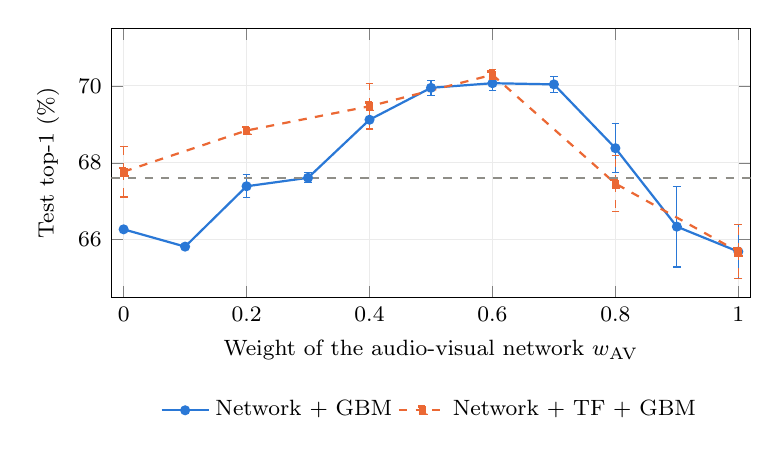
\begin{tikzpicture}
\begin{axis}[width=0.8\textwidth, height=5cm, xmin=-0.02, xmax=1.02, ymin=64.5, ymax=71.5,
  xlabel={Weight of the audio-visual network $w_{\mathrm{AV}}$}, ylabel={Test top-1 (\%)},
  label style={font=\footnotesize}, tick label style={font=\footnotesize}, legend style={font=\footnotesize, at={(0.5,-0.34)}, anchor=north, draw=none, legend columns=2},
  grid=major, grid style={draw=black!8}, error bars/y dir=both, error bars/y explicit]
\addplot[color=ours, mark=*, mark size=1.4pt, thick] coordinates {
 (0.0,66.27) +- (0,0) (0.1,65.82) +- (0,0.04) (0.2,67.39) +- (0,0.30) (0.3,67.61) +- (0,0.13) (0.4,69.12) +- (0,0.05)
 (0.5,69.95) +- (0,0.20) (0.6,70.07) +- (0,0.18) (0.7,70.04) +- (0,0.20) (0.8,68.38) +- (0,0.64) (0.9,66.34) +- (0,1.05) (1.0,65.69) +- (0,0.71)};
\addlegendentry{Network + GBM}
\addplot[color=fused, mark=square*, mark size=1.4pt, thick, dashed] coordinates {
 (0.0,67.77) +- (0,0.66) (0.2,68.84) +- (0,0.08) (0.4,69.47) +- (0,0.59) (0.6,70.29) +- (0,0.14) (0.8,67.46) +- (0,0.73) (1.0,65.69) +- (0,0.71)};
\addlegendentry{Network + TF + GBM}
\draw[dashed, published, thick] (axis cs:-0.02,67.61) -- (axis cs:1.02,67.61);
\end{axis}
\end{tikzpicture}
\caption{Sensitivity of the fused test top-1 accuracy to the fusion weights (mean $\pm$ standard deviation over three seeds; thresholds fitted on validation for every weight). The remaining weight $1 - w_{\mathrm{AV}}$ goes to the gradient-boosting model, or is split equally between the segment Transformer and the gradient-boosting model. The dashed grey line is the best published test result (67.61\%). At $w_{\mathrm{AV}} = 1$ the three network seeds are decoded with the fusion threshold search, which gives a mean of 65.69\% instead of the 66.27\% of their own refined thresholds}
\label{fig:sensitivity}
\end{figure}

\section{Computational cost}\label{sec:s_cost}

Table~\ref{tab:cost} reports the size and inference cost of every component of \ournet{} (Section~5.5 of the main text).

\begin{table}[t]
\setlength{\tabcolsep}{3pt}
\caption{Size and inference cost per 10\,s clip (batch size 1). GPU: NVIDIA RTX 3090; CPU timings use eight threads except OpenFace, which runs on one thread (median over 30 test clips; GPU time 21.5 $\pm$ 5.1\,ms). FLOPs count one multiply-add as two operations}\label{tab:cost}
\begin{tabular*}{0.8\textwidth}{@{\extracolsep\fill}lccl}
\toprule
Component & Params & FLOPs & Time\\
\midrule
Audio-visual network & 2.38\,M & 16.0\,G & 21.5\,ms GPU\\
 & & & 271\,ms CPU\\
\quad Frame encoder & 1.26\,M & -- & --\\
\quad Audio encoder & 0.27\,M & -- & --\\
\quad Cross-attention & 0.55\,M & 0.04\,G & --\\
Segment Transformer & 71.6\,k & 0.11\,M & 0.7\,ms CPU\\
Gradient boosting & 4.8\,k trees & -- & 38.6\,ms CPU\\
OpenFace 2.2 & -- & -- & 11.3\,s CPU\\
\botrule
\end{tabular*}
\end{table}

\section{Label granularity}\label{sec:s_gran}

Table~\ref{tab:granularity} shows the effect of merging engagement levels in the output of one trained audio-visual network without retraining (Section~5.6 of the main text).

\begin{table}[t]
\caption{Effect of label granularity on the output of one audio-visual network (seed 3, argmax, no retraining; test top-1 and majority-class accuracy in \%)}\label{tab:granularity}
\begin{tabular*}{0.6\textwidth}{@{\extracolsep\fill}lccc}
\toprule
Levels & Top-1 & Majority & Gain\\
\midrule
4 (as trained) & 64.27 & 50.27 & +14.00\\
3 (middle two merged) & 70.70 & 50.27 & \textbf{+20.43}\\
2 (0--1 vs.\ 2--3) & 85.95 & 68.84 & +17.11\\
\botrule
\end{tabular*}
\end{table}


\section{Training configuration}\label{sec:s_config}

Table~\ref{tab:config} lists the training configuration of the three models of \ournet{} (Section~4.3 of the main text).

\begin{table}[t]
\caption{Training configuration of the three models}\label{tab:config}
\begin{tabular*}{\textwidth}{@{\extracolsep\fill}llll}
\toprule
Setting & Audio-visual network & Segment Transformer & Gradient boosting\\
\midrule
Input & 50 face frames + log-mel & 20 tokens (44-d) & 924-d vector\\
Optimizer & SGD, momentum 0.9 & AdamW & --\\
Learning rate & $5 \times 10^{-5}$, constant & $10^{-3}$, warm-up cosine & 0.05 / 0.03 / 0.05\\
Weight decay / L2 & $10^{-3}$ & 0.05 & 1.0\\
Batch size & 8 & 64 & --\\
Epochs / iterations & 6 (fine-tuning) & 60 & 300 / 600 / 300\\
Loss & CE + ordinal & CE + ordinal & log loss\\
Ordinal weight $\lambda$ & 0.15 & 0.15 & --\\
Label smoothing & 0.1 & 0.1 & --\\
Sampling & inverse-sqrt class frequency & uniform & uniform\\
Dropout & modality 0.15 & 0.3, token 0.1 & --\\
Tree size & -- & -- & $\le$ 15 leaves\\
Seeds & 3 & 3 & 3 fits averaged\\
\botrule
\end{tabular*}
\end{table}

\section{Per-level results}\label{sec:s_levels}

Table~\ref{tab:levels} reports precision, recall and F1 per engagement level for each model on the test split (Section~5.2 of the main text).

\begin{table}[t]
\caption{Precision (P), recall (R) and F1 per engagement level on the test split (\%, mean of three seeds)}\label{tab:levels}
\setlength{\tabcolsep}{3pt}
\begin{tabular*}{\textwidth}{@{\extracolsep\fill}lcccccccccccc}
\toprule
& \multicolumn{3}{c}{Not engaged} & \multicolumn{3}{c}{Barely engaged} & \multicolumn{3}{c}{Engaged} & \multicolumn{3}{c}{Highly engaged}\\
\cmidrule{2-4}\cmidrule{5-7}\cmidrule{8-10}\cmidrule{11-13}
Model & P & R & F1 & P & R & F1 & P & R & F1 & P & R & F1\\
\midrule
Audio-visual network & 78.9 & 76.8 & \textbf{77.8} & 30.6 & 17.8 & \textbf{22.3} & 32.5 & 25.9 & 28.8 & 74.3 & 87.4 & 80.3\\
Gradient boosting & 71.3 & 67.4 & 69.3 & 44.4 & 1.6 & 3.1 & 37.5 & 59.4 & \textbf{46.0} & 81.1 & 82.4 & 81.8\\
Segment Transformer & 63.2 & 68.9 & 65.9 & 23.0 & 5.1 & 8.4 & 40.6 & 39.2 & 39.7 & 78.6 & 89.9 & 83.8\\
\ournet & 78.5 & 73.0 & 75.5 & 32.4 & 10.6 & 15.4 & 42.1 & 37.7 & 39.8 & 77.6 & 94.2 & \textbf{85.1}\\
\botrule
\end{tabular*}
\end{table}

\section{Behavior branch inside the network}\label{sec:s_branch}

Table~\ref{tab:branch} gives the four metrics of the behavior-branch ablation (Section~5.4.2 of the main text).

\begin{table}[t]
\caption{Behavior branch inside the network (test, three seeds). AV: the audio-visual network; + branch: with the behavior branch; + AU text: with the branch and the action-unit text}\label{tab:branch}
\begin{tabular*}{0.6\textwidth}{@{\extracolsep\fill}lccc}
\toprule
Metric & AV & + branch & + AU text\\
\midrule
Top-1 & \textbf{66.27$\pm$0.45} & 66.08$\pm$0.59 & 66.12$\pm$0.59\\
Adj. & 91.55 & 91.62 & \textbf{91.67}\\
MAE & 0.440 & 0.441 & \textbf{0.439}\\
Macro-F1 & \textbf{52.31} & 52.16 & 52.26\\
\botrule
\end{tabular*}
\end{table}

\section{Dataset statistics}\label{sec:s_dataset}

Table~\ref{tab:dataset} gives the number of EngageNet clips of each engagement level in the three splits (Section~4.1 of the main text).

\begin{table}[t]
\caption{EngageNet clips used in this work, by engagement level (0 not engaged, 1 barely engaged, 2 engaged, 3 highly engaged). The last column is the share of each level in the test split}\label{tab:dataset}
\begin{tabular*}{0.6\textwidth}{@{\extracolsep\fill}lrrrr}
\toprule
 & Train & Val. & Test & Test (\%)\\
\midrule
Participants & 90 & 11 & 26 & \\
Clips & 7,879 & 1,071 & 2,256 & \\
\midrule
Level 0 & 1,446 & 132 & 457 & 20.3\\
Level 1 & 1,035 & 97 & 246 & 10.9\\
Level 2 & 1,658 & 273 & 419 & 18.6\\
Level 3 & 3,740 & 569 & 1,134 & 50.3\\
\botrule
\end{tabular*}
\end{table}

\section{Modality and fusion-weight ablation tables}\label{sec:s_modfus}

Table~\ref{tab:modality} summarizes the inference-time modality ablation (Section~5.4.1 of the main text) and Table~\ref{tab:fusion} the late fusion under different weight rules (Section~5.4.3).

\begin{table}[t]
\caption{Inference-time modality ablation on the same trained weights (nine networks, test top-1, \%)}\label{tab:modality}
\begin{tabular*}{0.6\textwidth}{@{\extracolsep\fill}lcc}
\toprule
Input at inference & Mean top-1 & A+V higher in\\
\midrule
Audio + video & \textbf{66.16} & --\\
Video only & 65.41 & 7 of 9 (1 tie)\\
Audio only & 48.60 & 9 of 9\\
\botrule
\end{tabular*}
\end{table}

\begin{table}[t]
\caption{Late fusion under different weight rules (test top-1, \%, three seeds). AV: audio-visual network; TF: segment Transformer; GBM: gradient boosting}\label{tab:fusion}
\begin{tabular*}{0.6\textwidth}{@{\extracolsep\fill}llc}
\toprule
Members & Weight rule & Top-1\\
\midrule
AV + GBM & 0.5 / 0.5 & 69.95 $\pm$ 0.20\\
AV + GBM & 0.7 / 0.3 & 70.04 $\pm$ 0.20\\
AV + GBM & validation-selected & 69.86 $\pm$ 0.50\\
AV + TF + GBM & equal thirds & 69.28 $\pm$ 0.23\\
AV + TF + GBM & \textbf{0.6 / 0.2 / 0.2} & \textbf{70.29 $\pm$ 0.14}\\
AV + TF + GBM & validation-selected & 69.43--70.29\\
\botrule
\end{tabular*}
\end{table}

\end{document}
